% Created by tikzDevice version 0.12.3 on 2020-12-22 01:51:53
% !TEX encoding = UTF-8 Unicode
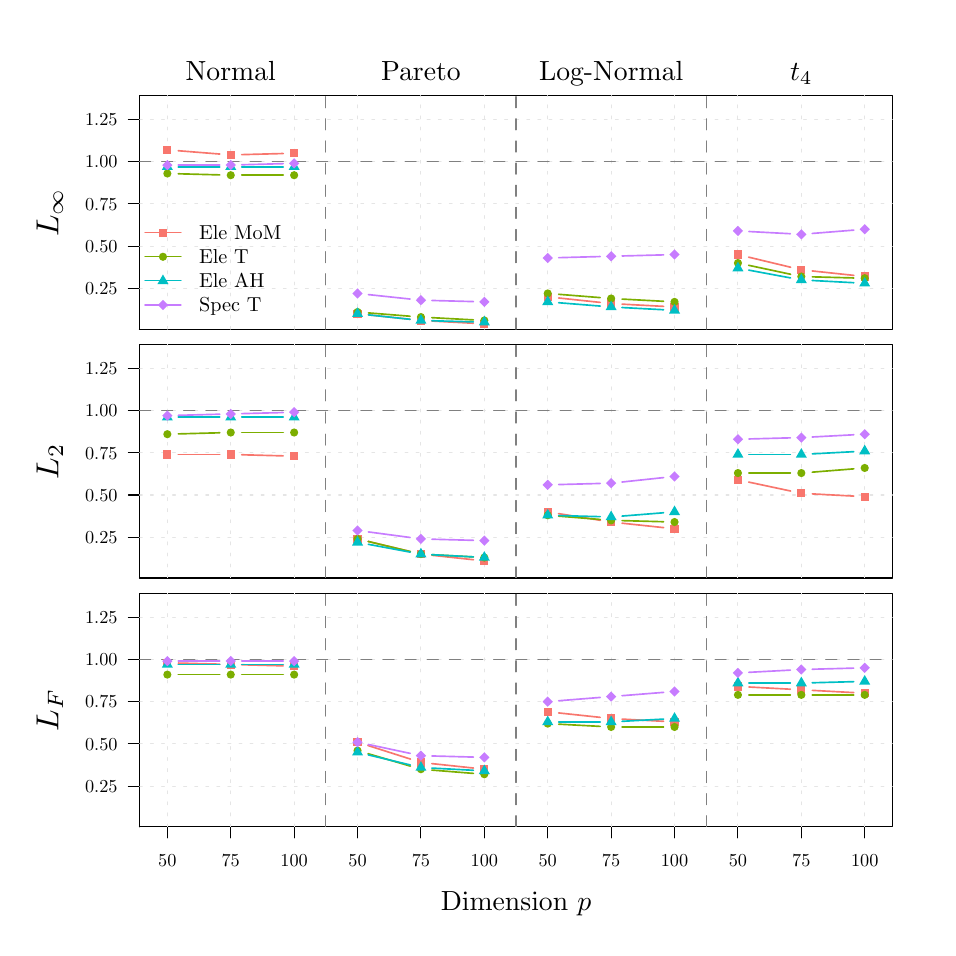
\begin{tikzpicture}[x=1pt,y=1pt]
\definecolor{fillColor}{RGB}{255,255,255}
\path[use as bounding box,fill=fillColor,fill opacity=0.00] (0,0) rectangle (325.21,325.21);
\begin{scope}
\path[clip] (  0.00,  0.00) rectangle (325.21,325.21);
\definecolor{drawColor}{RGB}{0,0,0}

\path[draw=drawColor,line width= 0.4pt,line join=round,line cap=round] ( 40.39,216.28) --
	(312.54,216.28) --
	(312.54,300.66) --
	( 40.39,300.66) --
	( 40.39,216.28);

\path[draw=drawColor,line width= 0.4pt,line join=round,line cap=round] ( 40.39,231.00) -- ( 40.39,292.04);

\path[draw=drawColor,line width= 0.4pt,line join=round,line cap=round] ( 40.39,231.00) -- ( 36.43,231.00);

\path[draw=drawColor,line width= 0.4pt,line join=round,line cap=round] ( 40.39,246.26) -- ( 36.43,246.26);

\path[draw=drawColor,line width= 0.4pt,line join=round,line cap=round] ( 40.39,261.52) -- ( 36.43,261.52);

\path[draw=drawColor,line width= 0.4pt,line join=round,line cap=round] ( 40.39,276.78) -- ( 36.43,276.78);

\path[draw=drawColor,line width= 0.4pt,line join=round,line cap=round] ( 40.39,292.04) -- ( 36.43,292.04);

\node[text=drawColor,anchor=base east,inner sep=0pt, outer sep=0pt, scale=  0.66] at ( 32.47,228.73) {0.25};

\node[text=drawColor,anchor=base east,inner sep=0pt, outer sep=0pt, scale=  0.66] at ( 32.47,243.99) {0.50};

\node[text=drawColor,anchor=base east,inner sep=0pt, outer sep=0pt, scale=  0.66] at ( 32.47,259.25) {0.75};

\node[text=drawColor,anchor=base east,inner sep=0pt, outer sep=0pt, scale=  0.66] at ( 32.47,274.51) {1.00};

\node[text=drawColor,anchor=base east,inner sep=0pt, outer sep=0pt, scale=  0.66] at ( 32.47,289.77) {1.25};
\end{scope}
\begin{scope}
\path[clip] ( 40.39,216.28) rectangle (312.54,300.66);
\definecolor{drawColor}{gray}{0.90}

\path[draw=drawColor,line width= 0.4pt,dash pattern=on 1pt off 3pt ,line join=round,line cap=round] ( 40.39,231.00) -- (312.54,231.00);

\path[draw=drawColor,line width= 0.4pt,dash pattern=on 1pt off 3pt ,line join=round,line cap=round] ( 40.39,246.26) -- (312.54,246.26);

\path[draw=drawColor,line width= 0.4pt,dash pattern=on 1pt off 3pt ,line join=round,line cap=round] ( 40.39,261.52) -- (312.54,261.52);

\path[draw=drawColor,line width= 0.4pt,dash pattern=on 1pt off 3pt ,line join=round,line cap=round] ( 40.39,276.78) -- (312.54,276.78);

\path[draw=drawColor,line width= 0.4pt,dash pattern=on 1pt off 3pt ,line join=round,line cap=round] ( 40.39,292.04) -- (312.54,292.04);

\path[draw=drawColor,line width= 0.4pt,dash pattern=on 1pt off 3pt ,line join=round,line cap=round] ( 50.47,216.28) -- ( 50.47,300.66);

\path[draw=drawColor,line width= 0.4pt,dash pattern=on 1pt off 3pt ,line join=round,line cap=round] ( 73.38,216.28) -- ( 73.38,300.66);

\path[draw=drawColor,line width= 0.4pt,dash pattern=on 1pt off 3pt ,line join=round,line cap=round] ( 96.29,216.28) -- ( 96.29,300.66);

\path[draw=drawColor,line width= 0.4pt,dash pattern=on 1pt off 3pt ,line join=round,line cap=round] (119.20,216.28) -- (119.20,300.66);

\path[draw=drawColor,line width= 0.4pt,dash pattern=on 1pt off 3pt ,line join=round,line cap=round] (142.10,216.28) -- (142.10,300.66);

\path[draw=drawColor,line width= 0.4pt,dash pattern=on 1pt off 3pt ,line join=round,line cap=round] (165.01,216.28) -- (165.01,300.66);

\path[draw=drawColor,line width= 0.4pt,dash pattern=on 1pt off 3pt ,line join=round,line cap=round] (187.92,216.28) -- (187.92,300.66);

\path[draw=drawColor,line width= 0.4pt,dash pattern=on 1pt off 3pt ,line join=round,line cap=round] (210.83,216.28) -- (210.83,300.66);

\path[draw=drawColor,line width= 0.4pt,dash pattern=on 1pt off 3pt ,line join=round,line cap=round] (233.74,216.28) -- (233.74,300.66);

\path[draw=drawColor,line width= 0.4pt,dash pattern=on 1pt off 3pt ,line join=round,line cap=round] (256.65,216.28) -- (256.65,300.66);

\path[draw=drawColor,line width= 0.4pt,dash pattern=on 1pt off 3pt ,line join=round,line cap=round] (279.56,216.28) -- (279.56,300.66);

\path[draw=drawColor,line width= 0.4pt,dash pattern=on 1pt off 3pt ,line join=round,line cap=round] (302.46,216.28) -- (302.46,300.66);
\definecolor{drawColor}{gray}{0.50}

\path[draw=drawColor,line width= 0.4pt,dash pattern=on 4pt off 4pt ,line join=round,line cap=round] (107.74,216.28) -- (107.74,300.66);

\path[draw=drawColor,line width= 0.4pt,dash pattern=on 4pt off 4pt ,line join=round,line cap=round] (176.47,216.28) -- (176.47,300.66);

\path[draw=drawColor,line width= 0.4pt,dash pattern=on 4pt off 4pt ,line join=round,line cap=round] (245.19,216.28) -- (245.19,300.66);

\path[draw=drawColor,line width= 0.4pt,dash pattern=on 4pt off 4pt ,line join=round,line cap=round] (313.92,216.28) -- (313.92,300.66);
\end{scope}
\begin{scope}
\path[clip] (  0.00,  0.00) rectangle (325.21,325.21);
\definecolor{drawColor}{RGB}{0,0,0}

\node[text=drawColor,rotate= 90.00,anchor=base,inner sep=0pt, outer sep=0pt, scale=  1.15] at ( 11.09,258.47) {$L_{\infty}$};
\end{scope}
\begin{scope}
\path[clip] ( 40.39,216.28) rectangle (312.54,300.66);
\definecolor{drawColor}{gray}{0.50}

\path[draw=drawColor,line width= 0.4pt,dash pattern=on 4pt off 4pt ,line join=round,line cap=round] ( 40.39,276.78) -- (312.54,276.78);
\end{scope}
\begin{scope}
\path[clip] (  0.00,  0.00) rectangle (325.21,325.21);
\definecolor{drawColor}{RGB}{0,0,0}

\node[text=drawColor,anchor=base,inner sep=0pt, outer sep=0pt, scale=  1.00] at ( 73.38,306.21) {Normal};

\node[text=drawColor,anchor=base,inner sep=0pt, outer sep=0pt, scale=  1.00] at (142.10,306.21) {Pareto};

\node[text=drawColor,anchor=base,inner sep=0pt, outer sep=0pt, scale=  1.00] at (210.83,306.21) {Log-Normal};

\node[text=drawColor,anchor=base,inner sep=0pt, outer sep=0pt, scale=  1.00] at (279.56,306.21) {$t_4$};
\end{scope}
\begin{scope}
\path[clip] ( 40.39,216.28) rectangle (312.54,300.66);
\definecolor{drawColor}{RGB}{248,118,109}

\path[draw=drawColor,line width= 0.4pt,line join=round,line cap=round] ( 42.35,251.13) -- ( 55.42,251.13);
\definecolor{drawColor}{RGB}{124,174,0}

\path[draw=drawColor,line width= 0.4pt,line join=round,line cap=round] ( 42.35,242.42) -- ( 55.42,242.42);
\definecolor{drawColor}{RGB}{0,191,196}

\path[draw=drawColor,line width= 0.4pt,line join=round,line cap=round] ( 42.35,233.71) -- ( 55.42,233.71);
\definecolor{drawColor}{RGB}{199,124,255}

\path[draw=drawColor,line width= 0.4pt,line join=round,line cap=round] ( 42.35,224.99) -- ( 55.42,224.99);
\definecolor{fillColor}{RGB}{248,118,109}

\path[fill=fillColor] ( 47.40,249.64) --
	( 50.37,249.64) --
	( 50.37,252.61) --
	( 47.40,252.61) --
	cycle;
\definecolor{fillColor}{RGB}{124,174,0}

\path[fill=fillColor] ( 48.89,242.42) circle (  1.48);
\definecolor{fillColor}{RGB}{0,191,196}

\path[fill=fillColor] ( 48.89,236.02) --
	( 50.89,232.55) --
	( 46.89,232.55) --
	cycle;
\definecolor{fillColor}{RGB}{199,124,255}

\path[fill=fillColor] ( 47.03,224.99) --
	( 48.89,226.85) --
	( 50.74,224.99) --
	( 48.89,223.14) --
	cycle;
\definecolor{drawColor}{RGB}{0,0,0}

\node[text=drawColor,anchor=base west,inner sep=0pt, outer sep=0pt, scale=  0.73] at ( 61.95,248.63) {Ele MoM};

\node[text=drawColor,anchor=base west,inner sep=0pt, outer sep=0pt, scale=  0.73] at ( 61.95,239.92) {Ele T};

\node[text=drawColor,anchor=base west,inner sep=0pt, outer sep=0pt, scale=  0.73] at ( 61.95,231.21) {Ele AH};

\node[text=drawColor,anchor=base west,inner sep=0pt, outer sep=0pt, scale=  0.73] at ( 61.95,222.49) {Spec T};
\definecolor{drawColor}{RGB}{248,118,109}

\path[draw=drawColor,line width= 0.6pt,line join=round,line cap=round] ( 54.42,280.74) -- ( 69.43,279.54);

\path[draw=drawColor,line width= 0.6pt,line join=round,line cap=round] ( 77.34,279.33) -- ( 92.33,279.73);
\definecolor{fillColor}{RGB}{248,118,109}

\path[fill=fillColor] ( 48.99,279.57) --
	( 51.96,279.57) --
	( 51.96,282.54) --
	( 48.99,282.54) --
	cycle;

\path[fill=fillColor] ( 71.89,277.74) --
	( 74.86,277.74) --
	( 74.86,280.71) --
	( 71.89,280.71) --
	cycle;

\path[fill=fillColor] ( 94.80,278.35) --
	( 97.77,278.35) --
	( 97.77,281.32) --
	( 94.80,281.32) --
	cycle;
\definecolor{drawColor}{RGB}{124,174,0}

\path[draw=drawColor,line width= 0.6pt,line join=round,line cap=round] ( 54.43,272.41) -- ( 69.42,272.01);

\path[draw=drawColor,line width= 0.6pt,line join=round,line cap=round] ( 77.34,271.90) -- ( 92.33,271.90);
\definecolor{fillColor}{RGB}{124,174,0}

\path[fill=fillColor] ( 50.47,272.51) circle (  1.48);

\path[fill=fillColor] ( 73.38,271.90) circle (  1.48);

\path[fill=fillColor] ( 96.29,271.90) circle (  1.48);
\definecolor{drawColor}{RGB}{0,191,196}

\path[draw=drawColor,line width= 0.6pt,line join=round,line cap=round] ( 54.43,274.95) -- ( 69.42,274.95);

\path[draw=drawColor,line width= 0.6pt,line join=round,line cap=round] ( 77.34,274.95) -- ( 92.33,274.95);
\definecolor{fillColor}{RGB}{0,191,196}

\path[fill=fillColor] ( 50.47,277.26) --
	( 52.47,273.80) --
	( 48.47,273.80) --
	cycle;

\path[fill=fillColor] ( 73.38,277.26) --
	( 75.38,273.80) --
	( 71.38,273.80) --
	cycle;

\path[fill=fillColor] ( 96.29,277.26) --
	( 98.29,273.80) --
	( 94.29,273.80) --
	cycle;
\definecolor{drawColor}{RGB}{199,124,255}

\path[draw=drawColor,line width= 0.6pt,line join=round,line cap=round] ( 54.43,275.56) -- ( 69.42,275.56);

\path[draw=drawColor,line width= 0.6pt,line join=round,line cap=round] ( 77.34,275.67) -- ( 92.33,276.07);
\definecolor{fillColor}{RGB}{199,124,255}

\path[fill=fillColor] ( 48.62,275.56) --
	( 50.47,277.42) --
	( 52.33,275.56) --
	( 50.47,273.71) --
	cycle;

\path[fill=fillColor] ( 71.52,275.56) --
	( 73.38,277.42) --
	( 75.24,275.56) --
	( 73.38,273.71) --
	cycle;

\path[fill=fillColor] ( 94.43,276.17) --
	( 96.29,278.03) --
	( 98.14,276.17) --
	( 96.29,274.32) --
	cycle;
\definecolor{drawColor}{RGB}{248,118,109}

\path[draw=drawColor,line width= 0.6pt,line join=round,line cap=round] (123.13,221.43) -- (138.17,219.83);

\path[draw=drawColor,line width= 0.6pt,line join=round,line cap=round] (146.06,219.20) -- (161.06,218.40);
\definecolor{fillColor}{RGB}{248,118,109}

\path[fill=fillColor] (117.71,220.36) --
	(120.68,220.36) --
	(120.68,223.33) --
	(117.71,223.33) --
	cycle;

\path[fill=fillColor] (140.62,217.92) --
	(143.59,217.92) --
	(143.59,220.89) --
	(140.62,220.89) --
	cycle;

\path[fill=fillColor] (163.53,216.70) --
	(166.50,216.70) --
	(166.50,219.67) --
	(163.53,219.67) --
	cycle;
\definecolor{drawColor}{RGB}{124,174,0}

\path[draw=drawColor,line width= 0.6pt,line join=round,line cap=round] (123.14,222.14) -- (138.16,220.94);

\path[draw=drawColor,line width= 0.6pt,line join=round,line cap=round] (146.06,220.42) -- (161.06,219.62);
\definecolor{fillColor}{RGB}{124,174,0}

\path[fill=fillColor] (119.20,222.46) circle (  1.48);

\path[fill=fillColor] (142.10,220.63) circle (  1.48);

\path[fill=fillColor] (165.01,219.41) circle (  1.48);
\definecolor{drawColor}{RGB}{0,191,196}

\path[draw=drawColor,line width= 0.6pt,line join=round,line cap=round] (123.13,221.43) -- (138.17,219.83);

\path[draw=drawColor,line width= 0.6pt,line join=round,line cap=round] (146.06,219.30) -- (161.05,218.90);
\definecolor{fillColor}{RGB}{0,191,196}

\path[fill=fillColor] (119.20,224.16) --
	(121.20,220.69) --
	(117.20,220.69) --
	cycle;

\path[fill=fillColor] (142.10,221.72) --
	(144.10,218.25) --
	(140.11,218.25) --
	cycle;

\path[fill=fillColor] (165.01,221.11) --
	(167.01,217.64) --
	(163.01,217.64) --
	cycle;
\definecolor{drawColor}{RGB}{199,124,255}

\path[draw=drawColor,line width= 0.6pt,line join=round,line cap=round] (123.13,228.75) -- (138.17,227.15);

\path[draw=drawColor,line width= 0.6pt,line join=round,line cap=round] (146.06,226.63) -- (161.05,226.23);
\definecolor{fillColor}{RGB}{199,124,255}

\path[fill=fillColor] (117.34,229.17) --
	(119.20,231.03) --
	(121.05,229.17) --
	(119.20,227.32) --
	cycle;

\path[fill=fillColor] (140.25,226.73) --
	(142.10,228.59) --
	(143.96,226.73) --
	(142.10,224.88) --
	cycle;

\path[fill=fillColor] (163.16,226.12) --
	(165.01,227.98) --
	(166.87,226.12) --
	(165.01,224.27) --
	cycle;
\definecolor{drawColor}{RGB}{248,118,109}

\path[draw=drawColor,line width= 0.6pt,line join=round,line cap=round] (191.86,227.53) -- (206.89,225.93);

\path[draw=drawColor,line width= 0.6pt,line join=round,line cap=round] (214.78,225.30) -- (229.78,224.50);
\definecolor{fillColor}{RGB}{248,118,109}

\path[fill=fillColor] (186.44,226.47) --
	(189.41,226.47) --
	(189.41,229.44) --
	(186.44,229.44) --
	cycle;

\path[fill=fillColor] (209.34,224.03) --
	(212.31,224.03) --
	(212.31,227.00) --
	(209.34,227.00) --
	cycle;

\path[fill=fillColor] (232.25,222.81) --
	(235.22,222.81) --
	(235.22,225.78) --
	(232.25,225.78) --
	cycle;
\definecolor{drawColor}{RGB}{124,174,0}

\path[draw=drawColor,line width= 0.6pt,line join=round,line cap=round] (191.87,228.86) -- (206.88,227.66);

\path[draw=drawColor,line width= 0.6pt,line join=round,line cap=round] (214.78,227.13) -- (229.78,226.33);
\definecolor{fillColor}{RGB}{124,174,0}

\path[fill=fillColor] (187.92,229.17) circle (  1.48);

\path[fill=fillColor] (210.83,227.34) circle (  1.48);

\path[fill=fillColor] (233.74,226.12) circle (  1.48);
\definecolor{drawColor}{RGB}{0,191,196}

\path[draw=drawColor,line width= 0.6pt,line join=round,line cap=round] (191.87,225.81) -- (206.88,224.61);

\path[draw=drawColor,line width= 0.6pt,line join=round,line cap=round] (214.78,224.08) -- (229.78,223.28);
\definecolor{fillColor}{RGB}{0,191,196}

\path[fill=fillColor] (187.92,228.43) --
	(189.92,224.97) --
	(185.92,224.97) --
	cycle;

\path[fill=fillColor] (210.83,226.60) --
	(212.83,223.14) --
	(208.83,223.14) --
	cycle;

\path[fill=fillColor] (233.74,225.38) --
	(235.74,221.91) --
	(231.74,221.91) --
	cycle;
\definecolor{drawColor}{RGB}{199,124,255}

\path[draw=drawColor,line width= 0.6pt,line join=round,line cap=round] (191.88,242.10) -- (206.87,242.50);

\path[draw=drawColor,line width= 0.6pt,line join=round,line cap=round] (214.79,242.71) -- (229.78,243.11);
\definecolor{fillColor}{RGB}{199,124,255}

\path[fill=fillColor] (186.07,241.99) --
	(187.92,243.85) --
	(189.78,241.99) --
	(187.92,240.14) --
	cycle;

\path[fill=fillColor] (208.97,242.60) --
	(210.83,244.46) --
	(212.69,242.60) --
	(210.83,240.75) --
	cycle;

\path[fill=fillColor] (231.88,243.21) --
	(233.74,245.07) --
	(235.59,243.21) --
	(233.74,241.36) --
	cycle;
\definecolor{drawColor}{RGB}{248,118,109}

\path[draw=drawColor,line width= 0.6pt,line join=round,line cap=round] (260.50,242.29) -- (275.70,238.64);

\path[draw=drawColor,line width= 0.6pt,line join=round,line cap=round] (283.49,237.30) -- (298.53,235.70);
\definecolor{fillColor}{RGB}{248,118,109}

\path[fill=fillColor] (255.16,241.73) --
	(258.13,241.73) --
	(258.13,244.70) --
	(255.16,244.70) --
	cycle;

\path[fill=fillColor] (278.07,236.23) --
	(281.04,236.23) --
	(281.04,239.20) --
	(278.07,239.20) --
	cycle;

\path[fill=fillColor] (300.98,233.79) --
	(303.95,233.79) --
	(303.95,236.76) --
	(300.98,236.76) --
	cycle;
\definecolor{drawColor}{RGB}{124,174,0}

\path[draw=drawColor,line width= 0.6pt,line join=round,line cap=round] (260.52,239.34) -- (275.68,236.10);

\path[draw=drawColor,line width= 0.6pt,line join=round,line cap=round] (283.51,235.17) -- (298.50,234.77);
\definecolor{fillColor}{RGB}{124,174,0}

\path[fill=fillColor] (256.65,240.16) circle (  1.48);

\path[fill=fillColor] (279.56,235.28) circle (  1.48);

\path[fill=fillColor] (302.46,234.67) circle (  1.48);
\definecolor{drawColor}{RGB}{0,191,196}

\path[draw=drawColor,line width= 0.6pt,line join=round,line cap=round] (260.54,237.60) -- (275.66,234.78);

\path[draw=drawColor,line width= 0.6pt,line join=round,line cap=round] (283.51,233.85) -- (298.51,233.05);
\definecolor{fillColor}{RGB}{0,191,196}

\path[fill=fillColor] (256.65,240.64) --
	(258.65,237.17) --
	(254.65,237.17) --
	cycle;

\path[fill=fillColor] (279.56,236.37) --
	(281.55,232.90) --
	(277.56,232.90) --
	cycle;

\path[fill=fillColor] (302.46,235.15) --
	(304.46,231.68) --
	(300.46,231.68) --
	cycle;
\definecolor{drawColor}{RGB}{199,124,255}

\path[draw=drawColor,line width= 0.6pt,line join=round,line cap=round] (260.60,251.55) -- (275.60,250.75);

\path[draw=drawColor,line width= 0.6pt,line join=round,line cap=round] (283.50,250.85) -- (298.52,252.05);
\definecolor{fillColor}{RGB}{199,124,255}

\path[fill=fillColor] (254.79,251.76) --
	(256.65,253.61) --
	(258.50,251.76) --
	(256.65,249.90) --
	cycle;

\path[fill=fillColor] (277.70,250.54) --
	(279.56,252.39) --
	(281.41,250.54) --
	(279.56,248.68) --
	cycle;

\path[fill=fillColor] (300.61,252.37) --
	(302.46,254.22) --
	(304.32,252.37) --
	(302.46,250.51) --
	cycle;
\end{scope}
\begin{scope}
\path[clip] (  0.00,  0.00) rectangle (325.21,325.21);
\definecolor{drawColor}{RGB}{0,0,0}

\path[draw=drawColor,line width= 0.4pt,line join=round,line cap=round] ( 40.39,126.36) --
	(312.54,126.36) --
	(312.54,210.74) --
	( 40.39,210.74) --
	( 40.39,126.36);

\path[draw=drawColor,line width= 0.4pt,line join=round,line cap=round] ( 40.39,141.08) -- ( 40.39,202.12);

\path[draw=drawColor,line width= 0.4pt,line join=round,line cap=round] ( 40.39,141.08) -- ( 36.43,141.08);

\path[draw=drawColor,line width= 0.4pt,line join=round,line cap=round] ( 40.39,156.34) -- ( 36.43,156.34);

\path[draw=drawColor,line width= 0.4pt,line join=round,line cap=round] ( 40.39,171.60) -- ( 36.43,171.60);

\path[draw=drawColor,line width= 0.4pt,line join=round,line cap=round] ( 40.39,186.86) -- ( 36.43,186.86);

\path[draw=drawColor,line width= 0.4pt,line join=round,line cap=round] ( 40.39,202.12) -- ( 36.43,202.12);

\node[text=drawColor,anchor=base east,inner sep=0pt, outer sep=0pt, scale=  0.66] at ( 32.47,138.81) {0.25};

\node[text=drawColor,anchor=base east,inner sep=0pt, outer sep=0pt, scale=  0.66] at ( 32.47,154.07) {0.50};

\node[text=drawColor,anchor=base east,inner sep=0pt, outer sep=0pt, scale=  0.66] at ( 32.47,169.33) {0.75};

\node[text=drawColor,anchor=base east,inner sep=0pt, outer sep=0pt, scale=  0.66] at ( 32.47,184.59) {1.00};

\node[text=drawColor,anchor=base east,inner sep=0pt, outer sep=0pt, scale=  0.66] at ( 32.47,199.85) {1.25};
\end{scope}
\begin{scope}
\path[clip] ( 40.39,126.36) rectangle (312.54,210.74);
\definecolor{drawColor}{gray}{0.90}

\path[draw=drawColor,line width= 0.4pt,dash pattern=on 1pt off 3pt ,line join=round,line cap=round] ( 40.39,141.08) -- (312.54,141.08);

\path[draw=drawColor,line width= 0.4pt,dash pattern=on 1pt off 3pt ,line join=round,line cap=round] ( 40.39,156.34) -- (312.54,156.34);

\path[draw=drawColor,line width= 0.4pt,dash pattern=on 1pt off 3pt ,line join=round,line cap=round] ( 40.39,171.60) -- (312.54,171.60);

\path[draw=drawColor,line width= 0.4pt,dash pattern=on 1pt off 3pt ,line join=round,line cap=round] ( 40.39,186.86) -- (312.54,186.86);

\path[draw=drawColor,line width= 0.4pt,dash pattern=on 1pt off 3pt ,line join=round,line cap=round] ( 40.39,202.12) -- (312.54,202.12);

\path[draw=drawColor,line width= 0.4pt,dash pattern=on 1pt off 3pt ,line join=round,line cap=round] ( 50.47,126.36) -- ( 50.47,210.74);

\path[draw=drawColor,line width= 0.4pt,dash pattern=on 1pt off 3pt ,line join=round,line cap=round] ( 73.38,126.36) -- ( 73.38,210.74);

\path[draw=drawColor,line width= 0.4pt,dash pattern=on 1pt off 3pt ,line join=round,line cap=round] ( 96.29,126.36) -- ( 96.29,210.74);

\path[draw=drawColor,line width= 0.4pt,dash pattern=on 1pt off 3pt ,line join=round,line cap=round] (119.20,126.36) -- (119.20,210.74);

\path[draw=drawColor,line width= 0.4pt,dash pattern=on 1pt off 3pt ,line join=round,line cap=round] (142.10,126.36) -- (142.10,210.74);

\path[draw=drawColor,line width= 0.4pt,dash pattern=on 1pt off 3pt ,line join=round,line cap=round] (165.01,126.36) -- (165.01,210.74);

\path[draw=drawColor,line width= 0.4pt,dash pattern=on 1pt off 3pt ,line join=round,line cap=round] (187.92,126.36) -- (187.92,210.74);

\path[draw=drawColor,line width= 0.4pt,dash pattern=on 1pt off 3pt ,line join=round,line cap=round] (210.83,126.36) -- (210.83,210.74);

\path[draw=drawColor,line width= 0.4pt,dash pattern=on 1pt off 3pt ,line join=round,line cap=round] (233.74,126.36) -- (233.74,210.74);

\path[draw=drawColor,line width= 0.4pt,dash pattern=on 1pt off 3pt ,line join=round,line cap=round] (256.65,126.36) -- (256.65,210.74);

\path[draw=drawColor,line width= 0.4pt,dash pattern=on 1pt off 3pt ,line join=round,line cap=round] (279.56,126.36) -- (279.56,210.74);

\path[draw=drawColor,line width= 0.4pt,dash pattern=on 1pt off 3pt ,line join=round,line cap=round] (302.46,126.36) -- (302.46,210.74);
\definecolor{drawColor}{gray}{0.50}

\path[draw=drawColor,line width= 0.4pt,dash pattern=on 4pt off 4pt ,line join=round,line cap=round] (107.74,126.36) -- (107.74,210.74);

\path[draw=drawColor,line width= 0.4pt,dash pattern=on 4pt off 4pt ,line join=round,line cap=round] (176.47,126.36) -- (176.47,210.74);

\path[draw=drawColor,line width= 0.4pt,dash pattern=on 4pt off 4pt ,line join=round,line cap=round] (245.19,126.36) -- (245.19,210.74);

\path[draw=drawColor,line width= 0.4pt,dash pattern=on 4pt off 4pt ,line join=round,line cap=round] (313.92,126.36) -- (313.92,210.74);
\end{scope}
\begin{scope}
\path[clip] (  0.00,  0.00) rectangle (325.21,325.21);
\definecolor{drawColor}{RGB}{0,0,0}

\node[text=drawColor,rotate= 90.00,anchor=base,inner sep=0pt, outer sep=0pt, scale=  1.15] at ( 11.09,168.55) {$L_{2}$};
\end{scope}
\begin{scope}
\path[clip] ( 40.39,126.36) rectangle (312.54,210.74);
\definecolor{drawColor}{gray}{0.50}

\path[draw=drawColor,line width= 0.4pt,dash pattern=on 4pt off 4pt ,line join=round,line cap=round] ( 40.39,186.86) -- (312.54,186.86);
\definecolor{drawColor}{RGB}{248,118,109}

\path[draw=drawColor,line width= 0.6pt,line join=round,line cap=round] ( 54.43,170.99) -- ( 69.42,170.99);

\path[draw=drawColor,line width= 0.6pt,line join=round,line cap=round] ( 77.34,170.88) -- ( 92.33,170.48);
\definecolor{fillColor}{RGB}{248,118,109}

\path[fill=fillColor] ( 48.99,169.50) --
	( 51.96,169.50) --
	( 51.96,172.47) --
	( 48.99,172.47) --
	cycle;

\path[fill=fillColor] ( 71.89,169.50) --
	( 74.86,169.50) --
	( 74.86,172.47) --
	( 71.89,172.47) --
	cycle;

\path[fill=fillColor] ( 94.80,168.89) --
	( 97.77,168.89) --
	( 97.77,171.86) --
	( 94.80,171.86) --
	cycle;
\definecolor{drawColor}{RGB}{124,174,0}

\path[draw=drawColor,line width= 0.6pt,line join=round,line cap=round] ( 54.43,178.42) -- ( 69.42,178.82);

\path[draw=drawColor,line width= 0.6pt,line join=round,line cap=round] ( 77.34,178.92) -- ( 92.33,178.92);
\definecolor{fillColor}{RGB}{124,174,0}

\path[fill=fillColor] ( 50.47,178.31) circle (  1.48);

\path[fill=fillColor] ( 73.38,178.92) circle (  1.48);

\path[fill=fillColor] ( 96.29,178.92) circle (  1.48);
\definecolor{drawColor}{RGB}{0,191,196}

\path[draw=drawColor,line width= 0.6pt,line join=round,line cap=round] ( 54.43,184.42) -- ( 69.42,184.42);

\path[draw=drawColor,line width= 0.6pt,line join=round,line cap=round] ( 77.34,184.42) -- ( 92.33,184.42);
\definecolor{fillColor}{RGB}{0,191,196}

\path[fill=fillColor] ( 50.47,186.73) --
	( 52.47,183.26) --
	( 48.47,183.26) --
	cycle;

\path[fill=fillColor] ( 73.38,186.73) --
	( 75.38,183.26) --
	( 71.38,183.26) --
	cycle;

\path[fill=fillColor] ( 96.29,186.73) --
	( 98.29,183.26) --
	( 94.29,183.26) --
	cycle;
\definecolor{drawColor}{RGB}{199,124,255}

\path[draw=drawColor,line width= 0.6pt,line join=round,line cap=round] ( 54.43,185.13) -- ( 69.42,185.53);

\path[draw=drawColor,line width= 0.6pt,line join=round,line cap=round] ( 77.34,185.74) -- ( 92.33,186.14);
\definecolor{fillColor}{RGB}{199,124,255}

\path[fill=fillColor] ( 48.62,185.03) --
	( 50.47,186.88) --
	( 52.33,185.03) --
	( 50.47,183.17) --
	cycle;

\path[fill=fillColor] ( 71.52,185.64) --
	( 73.38,187.49) --
	( 75.24,185.64) --
	( 73.38,183.78) --
	cycle;

\path[fill=fillColor] ( 94.43,186.25) --
	( 96.29,188.11) --
	( 98.14,186.25) --
	( 96.29,184.39) --
	cycle;
\definecolor{drawColor}{RGB}{248,118,109}

\path[draw=drawColor,line width= 0.6pt,line join=round,line cap=round] (123.05,139.55) -- (138.25,135.90);

\path[draw=drawColor,line width= 0.6pt,line join=round,line cap=round] (146.04,134.56) -- (161.08,132.95);
\definecolor{fillColor}{RGB}{248,118,109}

\path[fill=fillColor] (117.71,138.98) --
	(120.68,138.98) --
	(120.68,141.95) --
	(117.71,141.95) --
	cycle;

\path[fill=fillColor] (140.62,133.49) --
	(143.59,133.49) --
	(143.59,136.46) --
	(140.62,136.46) --
	cycle;

\path[fill=fillColor] (163.53,131.05) --
	(166.50,131.05) --
	(166.50,134.02) --
	(163.53,134.02) --
	cycle;
\definecolor{drawColor}{RGB}{124,174,0}

\path[draw=drawColor,line width= 0.6pt,line join=round,line cap=round] (123.05,139.55) -- (138.25,135.90);

\path[draw=drawColor,line width= 0.6pt,line join=round,line cap=round] (146.06,134.77) -- (161.06,133.97);
\definecolor{fillColor}{RGB}{124,174,0}

\path[fill=fillColor] (119.20,140.47) circle (  1.48);

\path[fill=fillColor] (142.10,134.98) circle (  1.48);

\path[fill=fillColor] (165.01,133.75) circle (  1.48);
\definecolor{drawColor}{RGB}{0,191,196}

\path[draw=drawColor,line width= 0.6pt,line join=round,line cap=round] (123.09,138.52) -- (138.21,135.70);

\path[draw=drawColor,line width= 0.6pt,line join=round,line cap=round] (146.06,134.77) -- (161.06,133.97);
\definecolor{fillColor}{RGB}{0,191,196}

\path[fill=fillColor] (119.20,141.56) --
	(121.20,138.09) --
	(117.20,138.09) --
	cycle;

\path[fill=fillColor] (142.10,137.29) --
	(144.10,133.82) --
	(140.11,133.82) --
	cycle;

\path[fill=fillColor] (165.01,136.06) --
	(167.01,132.60) --
	(163.01,132.60) --
	cycle;
\definecolor{drawColor}{RGB}{199,124,255}

\path[draw=drawColor,line width= 0.6pt,line join=round,line cap=round] (123.12,143.00) -- (138.18,140.99);

\path[draw=drawColor,line width= 0.6pt,line join=round,line cap=round] (146.06,140.36) -- (161.05,139.96);
\definecolor{fillColor}{RGB}{199,124,255}

\path[fill=fillColor] (117.34,143.52) --
	(119.20,145.38) --
	(121.05,143.52) --
	(119.20,141.67) --
	cycle;

\path[fill=fillColor] (140.25,140.47) --
	(142.10,142.33) --
	(143.96,140.47) --
	(142.10,138.61) --
	cycle;

\path[fill=fillColor] (163.16,139.86) --
	(165.01,141.72) --
	(166.87,139.86) --
	(165.01,138.00) --
	cycle;
\definecolor{drawColor}{RGB}{248,118,109}

\path[draw=drawColor,line width= 0.6pt,line join=round,line cap=round] (191.83,149.61) -- (206.92,147.20);

\path[draw=drawColor,line width= 0.6pt,line join=round,line cap=round] (214.77,146.15) -- (229.80,144.55);
\definecolor{fillColor}{RGB}{248,118,109}

\path[fill=fillColor] (186.44,148.75) --
	(189.41,148.75) --
	(189.41,151.72) --
	(186.44,151.72) --
	cycle;

\path[fill=fillColor] (209.34,145.09) --
	(212.31,145.09) --
	(212.31,148.06) --
	(209.34,148.06) --
	cycle;

\path[fill=fillColor] (232.25,142.65) --
	(235.22,142.65) --
	(235.22,145.62) --
	(232.25,145.62) --
	cycle;
\definecolor{drawColor}{RGB}{124,174,0}

\path[draw=drawColor,line width= 0.6pt,line join=round,line cap=round] (191.87,148.70) -- (206.88,147.50);

\path[draw=drawColor,line width= 0.6pt,line join=round,line cap=round] (214.79,147.08) -- (229.78,146.68);
\definecolor{fillColor}{RGB}{124,174,0}

\path[fill=fillColor] (187.92,149.01) circle (  1.48);

\path[fill=fillColor] (210.83,147.18) circle (  1.48);

\path[fill=fillColor] (233.74,146.57) circle (  1.48);
\definecolor{drawColor}{RGB}{0,191,196}

\path[draw=drawColor,line width= 0.6pt,line join=round,line cap=round] (191.88,148.91) -- (206.87,148.51);

\path[draw=drawColor,line width= 0.6pt,line join=round,line cap=round] (214.78,148.72) -- (229.79,149.92);
\definecolor{fillColor}{RGB}{0,191,196}

\path[fill=fillColor] (187.92,151.32) --
	(189.92,147.86) --
	(185.92,147.86) --
	cycle;

\path[fill=fillColor] (210.83,150.71) --
	(212.83,147.25) --
	(208.83,147.25) --
	cycle;

\path[fill=fillColor] (233.74,152.55) --
	(235.74,149.08) --
	(231.74,149.08) --
	cycle;
\definecolor{drawColor}{RGB}{199,124,255}

\path[draw=drawColor,line width= 0.6pt,line join=round,line cap=round] (191.88,160.11) -- (206.87,160.51);

\path[draw=drawColor,line width= 0.6pt,line join=round,line cap=round] (214.77,161.03) -- (229.80,162.63);
\definecolor{fillColor}{RGB}{199,124,255}

\path[fill=fillColor] (186.07,160.00) --
	(187.92,161.86) --
	(189.78,160.00) --
	(187.92,158.15) --
	cycle;

\path[fill=fillColor] (208.97,160.61) --
	(210.83,162.47) --
	(212.69,160.61) --
	(210.83,158.76) --
	cycle;

\path[fill=fillColor] (231.88,163.05) --
	(233.74,164.91) --
	(235.59,163.05) --
	(233.74,161.20) --
	cycle;
\definecolor{drawColor}{RGB}{248,118,109}

\path[draw=drawColor,line width= 0.6pt,line join=round,line cap=round] (260.52,161.01) -- (275.68,157.78);

\path[draw=drawColor,line width= 0.6pt,line join=round,line cap=round] (283.51,156.74) -- (298.51,155.94);
\definecolor{fillColor}{RGB}{248,118,109}

\path[fill=fillColor] (255.16,160.35) --
	(258.13,160.35) --
	(258.13,163.32) --
	(255.16,163.32) --
	cycle;

\path[fill=fillColor] (278.07,155.46) --
	(281.04,155.46) --
	(281.04,158.43) --
	(278.07,158.43) --
	cycle;

\path[fill=fillColor] (300.98,154.24) --
	(303.95,154.24) --
	(303.95,157.21) --
	(300.98,157.21) --
	cycle;
\definecolor{drawColor}{RGB}{124,174,0}

\path[draw=drawColor,line width= 0.6pt,line join=round,line cap=round] (260.61,164.27) -- (275.60,164.27);

\path[draw=drawColor,line width= 0.6pt,line join=round,line cap=round] (283.50,164.59) -- (298.52,165.79);
\definecolor{fillColor}{RGB}{124,174,0}

\path[fill=fillColor] (256.65,164.27) circle (  1.48);

\path[fill=fillColor] (279.56,164.27) circle (  1.48);

\path[fill=fillColor] (302.46,166.11) circle (  1.48);
\definecolor{drawColor}{RGB}{0,191,196}

\path[draw=drawColor,line width= 0.6pt,line join=round,line cap=round] (260.61,170.99) -- (275.60,170.99);

\path[draw=drawColor,line width= 0.6pt,line join=round,line cap=round] (283.51,171.20) -- (298.51,172.00);
\definecolor{fillColor}{RGB}{0,191,196}

\path[fill=fillColor] (256.65,173.30) --
	(258.65,169.83) --
	(254.65,169.83) --
	cycle;

\path[fill=fillColor] (279.56,173.30) --
	(281.55,169.83) --
	(277.56,169.83) --
	cycle;

\path[fill=fillColor] (302.46,174.52) --
	(304.46,171.06) --
	(300.46,171.06) --
	cycle;
\definecolor{drawColor}{RGB}{199,124,255}

\path[draw=drawColor,line width= 0.6pt,line join=round,line cap=round] (260.61,176.59) -- (275.60,176.99);

\path[draw=drawColor,line width= 0.6pt,line join=round,line cap=round] (283.51,177.30) -- (298.51,178.10);
\definecolor{fillColor}{RGB}{199,124,255}

\path[fill=fillColor] (254.79,176.48) --
	(256.65,178.34) --
	(258.50,176.48) --
	(256.65,174.63) --
	cycle;

\path[fill=fillColor] (277.70,177.09) --
	(279.56,178.95) --
	(281.41,177.09) --
	(279.56,175.24) --
	cycle;

\path[fill=fillColor] (300.61,178.31) --
	(302.46,180.17) --
	(304.32,178.31) --
	(302.46,176.46) --
	cycle;
\end{scope}
\begin{scope}
\path[clip] (  0.00,  0.00) rectangle (325.21,325.21);
\definecolor{drawColor}{RGB}{0,0,0}

\path[draw=drawColor,line width= 0.4pt,line join=round,line cap=round] ( 40.39, 36.43) --
	(312.54, 36.43) --
	(312.54,120.81) --
	( 40.39,120.81) --
	( 40.39, 36.43);

\path[draw=drawColor,line width= 0.4pt,line join=round,line cap=round] ( 40.39, 51.15) -- ( 40.39,112.19);

\path[draw=drawColor,line width= 0.4pt,line join=round,line cap=round] ( 40.39, 51.15) -- ( 36.43, 51.15);

\path[draw=drawColor,line width= 0.4pt,line join=round,line cap=round] ( 40.39, 66.41) -- ( 36.43, 66.41);

\path[draw=drawColor,line width= 0.4pt,line join=round,line cap=round] ( 40.39, 81.67) -- ( 36.43, 81.67);

\path[draw=drawColor,line width= 0.4pt,line join=round,line cap=round] ( 40.39, 96.93) -- ( 36.43, 96.93);

\path[draw=drawColor,line width= 0.4pt,line join=round,line cap=round] ( 40.39,112.19) -- ( 36.43,112.19);

\node[text=drawColor,anchor=base east,inner sep=0pt, outer sep=0pt, scale=  0.66] at ( 32.47, 48.88) {0.25};

\node[text=drawColor,anchor=base east,inner sep=0pt, outer sep=0pt, scale=  0.66] at ( 32.47, 64.14) {0.50};

\node[text=drawColor,anchor=base east,inner sep=0pt, outer sep=0pt, scale=  0.66] at ( 32.47, 79.40) {0.75};

\node[text=drawColor,anchor=base east,inner sep=0pt, outer sep=0pt, scale=  0.66] at ( 32.47, 94.66) {1.00};

\node[text=drawColor,anchor=base east,inner sep=0pt, outer sep=0pt, scale=  0.66] at ( 32.47,109.92) {1.25};
\end{scope}
\begin{scope}
\path[clip] ( 40.39, 36.43) rectangle (312.54,120.81);
\definecolor{drawColor}{gray}{0.90}

\path[draw=drawColor,line width= 0.4pt,dash pattern=on 1pt off 3pt ,line join=round,line cap=round] ( 40.39, 51.15) -- (312.54, 51.15);

\path[draw=drawColor,line width= 0.4pt,dash pattern=on 1pt off 3pt ,line join=round,line cap=round] ( 40.39, 66.41) -- (312.54, 66.41);

\path[draw=drawColor,line width= 0.4pt,dash pattern=on 1pt off 3pt ,line join=round,line cap=round] ( 40.39, 81.67) -- (312.54, 81.67);

\path[draw=drawColor,line width= 0.4pt,dash pattern=on 1pt off 3pt ,line join=round,line cap=round] ( 40.39, 96.93) -- (312.54, 96.93);

\path[draw=drawColor,line width= 0.4pt,dash pattern=on 1pt off 3pt ,line join=round,line cap=round] ( 40.39,112.19) -- (312.54,112.19);
\end{scope}
\begin{scope}
\path[clip] (  0.00,  0.00) rectangle (325.21,325.21);
\definecolor{drawColor}{RGB}{0,0,0}

\path[draw=drawColor,line width= 0.4pt,line join=round,line cap=round] ( 50.47, 36.43) -- (302.46, 36.43);

\path[draw=drawColor,line width= 0.4pt,line join=round,line cap=round] ( 50.47, 36.43) -- ( 50.47, 32.47);

\path[draw=drawColor,line width= 0.4pt,line join=round,line cap=round] ( 73.38, 36.43) -- ( 73.38, 32.47);

\path[draw=drawColor,line width= 0.4pt,line join=round,line cap=round] ( 96.29, 36.43) -- ( 96.29, 32.47);

\path[draw=drawColor,line width= 0.4pt,line join=round,line cap=round] (119.20, 36.43) -- (119.20, 32.47);

\path[draw=drawColor,line width= 0.4pt,line join=round,line cap=round] (142.10, 36.43) -- (142.10, 32.47);

\path[draw=drawColor,line width= 0.4pt,line join=round,line cap=round] (165.01, 36.43) -- (165.01, 32.47);

\path[draw=drawColor,line width= 0.4pt,line join=round,line cap=round] (187.92, 36.43) -- (187.92, 32.47);

\path[draw=drawColor,line width= 0.4pt,line join=round,line cap=round] (210.83, 36.43) -- (210.83, 32.47);

\path[draw=drawColor,line width= 0.4pt,line join=round,line cap=round] (233.74, 36.43) -- (233.74, 32.47);

\path[draw=drawColor,line width= 0.4pt,line join=round,line cap=round] (256.65, 36.43) -- (256.65, 32.47);

\path[draw=drawColor,line width= 0.4pt,line join=round,line cap=round] (279.56, 36.43) -- (279.56, 32.47);

\path[draw=drawColor,line width= 0.4pt,line join=round,line cap=round] (302.46, 36.43) -- (302.46, 32.47);

\node[text=drawColor,anchor=base,inner sep=0pt, outer sep=0pt, scale=  0.66] at ( 50.47, 22.18) {50};

\node[text=drawColor,anchor=base,inner sep=0pt, outer sep=0pt, scale=  0.66] at ( 73.38, 22.18) {75};

\node[text=drawColor,anchor=base,inner sep=0pt, outer sep=0pt, scale=  0.66] at ( 96.29, 22.18) {100};

\node[text=drawColor,anchor=base,inner sep=0pt, outer sep=0pt, scale=  0.66] at (119.20, 22.18) {50};

\node[text=drawColor,anchor=base,inner sep=0pt, outer sep=0pt, scale=  0.66] at (142.10, 22.18) {75};

\node[text=drawColor,anchor=base,inner sep=0pt, outer sep=0pt, scale=  0.66] at (165.01, 22.18) {100};

\node[text=drawColor,anchor=base,inner sep=0pt, outer sep=0pt, scale=  0.66] at (187.92, 22.18) {50};

\node[text=drawColor,anchor=base,inner sep=0pt, outer sep=0pt, scale=  0.66] at (210.83, 22.18) {75};

\node[text=drawColor,anchor=base,inner sep=0pt, outer sep=0pt, scale=  0.66] at (233.74, 22.18) {100};

\node[text=drawColor,anchor=base,inner sep=0pt, outer sep=0pt, scale=  0.66] at (256.65, 22.18) {50};

\node[text=drawColor,anchor=base,inner sep=0pt, outer sep=0pt, scale=  0.66] at (279.56, 22.18) {75};

\node[text=drawColor,anchor=base,inner sep=0pt, outer sep=0pt, scale=  0.66] at (302.46, 22.18) {100};
\end{scope}
\begin{scope}
\path[clip] ( 40.39, 36.43) rectangle (312.54,120.81);
\definecolor{drawColor}{gray}{0.90}

\path[draw=drawColor,line width= 0.4pt,dash pattern=on 1pt off 3pt ,line join=round,line cap=round] ( 50.47, 36.43) -- ( 50.47,120.81);

\path[draw=drawColor,line width= 0.4pt,dash pattern=on 1pt off 3pt ,line join=round,line cap=round] ( 73.38, 36.43) -- ( 73.38,120.81);

\path[draw=drawColor,line width= 0.4pt,dash pattern=on 1pt off 3pt ,line join=round,line cap=round] ( 96.29, 36.43) -- ( 96.29,120.81);

\path[draw=drawColor,line width= 0.4pt,dash pattern=on 1pt off 3pt ,line join=round,line cap=round] (119.20, 36.43) -- (119.20,120.81);

\path[draw=drawColor,line width= 0.4pt,dash pattern=on 1pt off 3pt ,line join=round,line cap=round] (142.10, 36.43) -- (142.10,120.81);

\path[draw=drawColor,line width= 0.4pt,dash pattern=on 1pt off 3pt ,line join=round,line cap=round] (165.01, 36.43) -- (165.01,120.81);

\path[draw=drawColor,line width= 0.4pt,dash pattern=on 1pt off 3pt ,line join=round,line cap=round] (187.92, 36.43) -- (187.92,120.81);

\path[draw=drawColor,line width= 0.4pt,dash pattern=on 1pt off 3pt ,line join=round,line cap=round] (210.83, 36.43) -- (210.83,120.81);

\path[draw=drawColor,line width= 0.4pt,dash pattern=on 1pt off 3pt ,line join=round,line cap=round] (233.74, 36.43) -- (233.74,120.81);

\path[draw=drawColor,line width= 0.4pt,dash pattern=on 1pt off 3pt ,line join=round,line cap=round] (256.65, 36.43) -- (256.65,120.81);

\path[draw=drawColor,line width= 0.4pt,dash pattern=on 1pt off 3pt ,line join=round,line cap=round] (279.56, 36.43) -- (279.56,120.81);

\path[draw=drawColor,line width= 0.4pt,dash pattern=on 1pt off 3pt ,line join=round,line cap=round] (302.46, 36.43) -- (302.46,120.81);
\definecolor{drawColor}{gray}{0.50}

\path[draw=drawColor,line width= 0.4pt,dash pattern=on 4pt off 4pt ,line join=round,line cap=round] (107.74, 36.43) -- (107.74,120.81);

\path[draw=drawColor,line width= 0.4pt,dash pattern=on 4pt off 4pt ,line join=round,line cap=round] (176.47, 36.43) -- (176.47,120.81);

\path[draw=drawColor,line width= 0.4pt,dash pattern=on 4pt off 4pt ,line join=round,line cap=round] (245.19, 36.43) -- (245.19,120.81);

\path[draw=drawColor,line width= 0.4pt,dash pattern=on 4pt off 4pt ,line join=round,line cap=round] (313.92, 36.43) -- (313.92,120.81);
\end{scope}
\begin{scope}
\path[clip] (  0.00,  0.00) rectangle (325.21,325.21);
\definecolor{drawColor}{RGB}{0,0,0}

\node[text=drawColor,rotate= 90.00,anchor=base,inner sep=0pt, outer sep=0pt, scale=  1.15] at ( 11.09, 78.62) {$L_{F}$};
\end{scope}
\begin{scope}
\path[clip] ( 40.39, 36.43) rectangle (312.54,120.81);
\definecolor{drawColor}{gray}{0.50}

\path[draw=drawColor,line width= 0.4pt,dash pattern=on 4pt off 4pt ,line join=round,line cap=round] ( 40.39, 96.93) -- (312.54, 96.93);
\end{scope}
\begin{scope}
\path[clip] (  0.00,  0.00) rectangle (325.21,325.21);
\definecolor{drawColor}{RGB}{0,0,0}

\node[text=drawColor,anchor=base,inner sep=0pt, outer sep=0pt, scale=  1.00] at (176.47,  6.34) {Dimension $p$};
\end{scope}
\begin{scope}
\path[clip] ( 40.39, 36.43) rectangle (312.54,120.81);
\definecolor{drawColor}{RGB}{248,118,109}

\path[draw=drawColor,line width= 0.6pt,line join=round,line cap=round] ( 54.43, 95.61) -- ( 69.42, 95.21);

\path[draw=drawColor,line width= 0.6pt,line join=round,line cap=round] ( 77.34, 95.00) -- ( 92.33, 94.60);
\definecolor{fillColor}{RGB}{248,118,109}

\path[fill=fillColor] ( 48.99, 94.23) --
	( 51.96, 94.23) --
	( 51.96, 97.20) --
	( 48.99, 97.20) --
	cycle;

\path[fill=fillColor] ( 71.89, 93.62) --
	( 74.86, 93.62) --
	( 74.86, 96.59) --
	( 71.89, 96.59) --
	cycle;

\path[fill=fillColor] ( 94.80, 93.01) --
	( 97.77, 93.01) --
	( 97.77, 95.98) --
	( 94.80, 95.98) --
	cycle;
\definecolor{drawColor}{RGB}{124,174,0}

\path[draw=drawColor,line width= 0.6pt,line join=round,line cap=round] ( 54.43, 91.44) -- ( 69.42, 91.44);

\path[draw=drawColor,line width= 0.6pt,line join=round,line cap=round] ( 77.34, 91.44) -- ( 92.33, 91.44);
\definecolor{fillColor}{RGB}{124,174,0}

\path[fill=fillColor] ( 50.47, 91.44) circle (  1.48);

\path[fill=fillColor] ( 73.38, 91.44) circle (  1.48);

\path[fill=fillColor] ( 96.29, 91.44) circle (  1.48);
\definecolor{drawColor}{RGB}{0,191,196}

\path[draw=drawColor,line width= 0.6pt,line join=round,line cap=round] ( 54.43, 95.10) -- ( 69.42, 95.10);

\path[draw=drawColor,line width= 0.6pt,line join=round,line cap=round] ( 77.34, 95.10) -- ( 92.33, 95.10);
\definecolor{fillColor}{RGB}{0,191,196}

\path[fill=fillColor] ( 50.47, 97.41) --
	( 52.47, 93.95) --
	( 48.47, 93.95) --
	cycle;

\path[fill=fillColor] ( 73.38, 97.41) --
	( 75.38, 93.95) --
	( 71.38, 93.95) --
	cycle;

\path[fill=fillColor] ( 96.29, 97.41) --
	( 98.29, 93.95) --
	( 94.29, 93.95) --
	cycle;
\definecolor{drawColor}{RGB}{199,124,255}

\path[draw=drawColor,line width= 0.6pt,line join=round,line cap=round] ( 54.43, 96.32) -- ( 69.42, 96.32);

\path[draw=drawColor,line width= 0.6pt,line join=round,line cap=round] ( 77.34, 96.32) -- ( 92.33, 96.32);
\definecolor{fillColor}{RGB}{199,124,255}

\path[fill=fillColor] ( 48.62, 96.32) --
	( 50.47, 98.18) --
	( 52.33, 96.32) --
	( 50.47, 94.47) --
	cycle;

\path[fill=fillColor] ( 71.52, 96.32) --
	( 73.38, 98.18) --
	( 75.24, 96.32) --
	( 73.38, 94.47) --
	cycle;

\path[fill=fillColor] ( 94.43, 96.32) --
	( 96.29, 98.18) --
	( 98.14, 96.32) --
	( 96.29, 94.47) --
	cycle;
\definecolor{drawColor}{RGB}{248,118,109}

\path[draw=drawColor,line width= 0.6pt,line join=round,line cap=round] (122.97, 65.82) -- (138.33, 60.91);

\path[draw=drawColor,line width= 0.6pt,line join=round,line cap=round] (146.04, 59.28) -- (161.08, 57.68);
\definecolor{fillColor}{RGB}{248,118,109}

\path[fill=fillColor] (117.71, 65.54) --
	(120.68, 65.54) --
	(120.68, 68.51) --
	(117.71, 68.51) --
	cycle;

\path[fill=fillColor] (140.62, 58.22) --
	(143.59, 58.22) --
	(143.59, 61.19) --
	(140.62, 61.19) --
	cycle;

\path[fill=fillColor] (163.53, 55.77) --
	(166.50, 55.77) --
	(166.50, 58.74) --
	(163.53, 58.74) --
	cycle;
\definecolor{drawColor}{RGB}{124,174,0}

\path[draw=drawColor,line width= 0.6pt,line join=round,line cap=round] (123.00, 62.86) -- (138.30, 58.37);

\path[draw=drawColor,line width= 0.6pt,line join=round,line cap=round] (146.05, 56.94) -- (161.07, 55.74);
\definecolor{fillColor}{RGB}{124,174,0}

\path[fill=fillColor] (119.20, 63.97) circle (  1.48);

\path[fill=fillColor] (142.10, 57.26) circle (  1.48);

\path[fill=fillColor] (165.01, 55.43) circle (  1.48);
\definecolor{drawColor}{RGB}{0,191,196}

\path[draw=drawColor,line width= 0.6pt,line join=round,line cap=round] (123.05, 62.44) -- (138.25, 58.79);

\path[draw=drawColor,line width= 0.6pt,line join=round,line cap=round] (146.06, 57.66) -- (161.06, 56.86);
\definecolor{fillColor}{RGB}{0,191,196}

\path[fill=fillColor] (119.20, 65.67) --
	(121.20, 62.21) --
	(117.20, 62.21) --
	cycle;

\path[fill=fillColor] (142.10, 60.18) --
	(144.10, 56.71) --
	(140.11, 56.71) --
	cycle;

\path[fill=fillColor] (165.01, 58.96) --
	(167.01, 55.49) --
	(163.01, 55.49) --
	cycle;
\definecolor{drawColor}{RGB}{199,124,255}

\path[draw=drawColor,line width= 0.6pt,line join=round,line cap=round] (123.07, 66.20) -- (138.23, 62.97);

\path[draw=drawColor,line width= 0.6pt,line join=round,line cap=round] (146.06, 62.04) -- (161.05, 61.64);
\definecolor{fillColor}{RGB}{199,124,255}

\path[fill=fillColor] (117.34, 67.02) --
	(119.20, 68.88) --
	(121.05, 67.02) --
	(119.20, 65.17) --
	cycle;

\path[fill=fillColor] (140.25, 62.14) --
	(142.10, 64.00) --
	(143.96, 62.14) --
	(142.10, 60.29) --
	cycle;

\path[fill=fillColor] (163.16, 61.53) --
	(165.01, 63.39) --
	(166.87, 61.53) --
	(165.01, 59.68) --
	cycle;
\definecolor{drawColor}{RGB}{248,118,109}

\path[draw=drawColor,line width= 0.6pt,line join=round,line cap=round] (191.86, 77.59) -- (206.89, 75.99);

\path[draw=drawColor,line width= 0.6pt,line join=round,line cap=round] (214.78, 75.36) -- (229.78, 74.56);
\definecolor{fillColor}{RGB}{248,118,109}

\path[fill=fillColor] (186.44, 76.53) --
	(189.41, 76.53) --
	(189.41, 79.50) --
	(186.44, 79.50) --
	cycle;

\path[fill=fillColor] (209.34, 74.09) --
	(212.31, 74.09) --
	(212.31, 77.06) --
	(209.34, 77.06) --
	cycle;

\path[fill=fillColor] (232.25, 72.86) --
	(235.22, 72.86) --
	(235.22, 75.83) --
	(232.25, 75.83) --
	cycle;
\definecolor{drawColor}{RGB}{124,174,0}

\path[draw=drawColor,line width= 0.6pt,line join=round,line cap=round] (191.88, 73.53) -- (206.88, 72.73);

\path[draw=drawColor,line width= 0.6pt,line join=round,line cap=round] (214.79, 72.52) -- (229.78, 72.52);
\definecolor{fillColor}{RGB}{124,174,0}

\path[fill=fillColor] (187.92, 73.74) circle (  1.48);

\path[fill=fillColor] (210.83, 72.52) circle (  1.48);

\path[fill=fillColor] (233.74, 72.52) circle (  1.48);
\definecolor{drawColor}{RGB}{0,191,196}

\path[draw=drawColor,line width= 0.6pt,line join=round,line cap=round] (191.88, 74.35) -- (206.87, 74.35);

\path[draw=drawColor,line width= 0.6pt,line join=round,line cap=round] (214.78, 74.56) -- (229.78, 75.36);
\definecolor{fillColor}{RGB}{0,191,196}

\path[fill=fillColor] (187.92, 76.66) --
	(189.92, 73.20) --
	(185.92, 73.20) --
	cycle;

\path[fill=fillColor] (210.83, 76.66) --
	(212.83, 73.20) --
	(208.83, 73.20) --
	cycle;

\path[fill=fillColor] (233.74, 77.88) --
	(235.74, 74.42) --
	(231.74, 74.42) --
	cycle;
\definecolor{drawColor}{RGB}{199,124,255}

\path[draw=drawColor,line width= 0.6pt,line join=round,line cap=round] (191.87, 81.99) -- (206.88, 83.19);

\path[draw=drawColor,line width= 0.6pt,line join=round,line cap=round] (214.78, 83.82) -- (229.79, 85.02);
\definecolor{fillColor}{RGB}{199,124,255}

\path[fill=fillColor] (186.07, 81.67) --
	(187.92, 83.53) --
	(189.78, 81.67) --
	(187.92, 79.82) --
	cycle;

\path[fill=fillColor] (208.97, 83.51) --
	(210.83, 85.36) --
	(212.69, 83.51) --
	(210.83, 81.65) --
	cycle;

\path[fill=fillColor] (231.88, 85.34) --
	(233.74, 87.19) --
	(235.59, 85.34) --
	(233.74, 83.48) --
	cycle;
\definecolor{drawColor}{RGB}{248,118,109}

\path[draw=drawColor,line width= 0.6pt,line join=round,line cap=round] (260.60, 86.96) -- (275.60, 86.16);

\path[draw=drawColor,line width= 0.6pt,line join=round,line cap=round] (283.51, 85.74) -- (298.51, 84.94);
\definecolor{fillColor}{RGB}{248,118,109}

\path[fill=fillColor] (255.16, 85.68) --
	(258.13, 85.68) --
	(258.13, 88.65) --
	(255.16, 88.65) --
	cycle;

\path[fill=fillColor] (278.07, 84.46) --
	(281.04, 84.46) --
	(281.04, 87.43) --
	(278.07, 87.43) --
	cycle;

\path[fill=fillColor] (300.98, 83.24) --
	(303.95, 83.24) --
	(303.95, 86.21) --
	(300.98, 86.21) --
	cycle;
\definecolor{drawColor}{RGB}{124,174,0}

\path[draw=drawColor,line width= 0.6pt,line join=round,line cap=round] (260.61, 84.12) -- (275.60, 84.12);

\path[draw=drawColor,line width= 0.6pt,line join=round,line cap=round] (283.52, 84.12) -- (298.50, 84.12);
\definecolor{fillColor}{RGB}{124,174,0}

\path[fill=fillColor] (256.65, 84.12) circle (  1.48);

\path[fill=fillColor] (279.56, 84.12) circle (  1.48);

\path[fill=fillColor] (302.46, 84.12) circle (  1.48);
\definecolor{drawColor}{RGB}{0,191,196}

\path[draw=drawColor,line width= 0.6pt,line join=round,line cap=round] (260.61, 88.39) -- (275.60, 88.39);

\path[draw=drawColor,line width= 0.6pt,line join=round,line cap=round] (283.51, 88.49) -- (298.50, 88.89);
\definecolor{fillColor}{RGB}{0,191,196}

\path[fill=fillColor] (256.65, 90.70) --
	(258.65, 87.23) --
	(254.65, 87.23) --
	cycle;

\path[fill=fillColor] (279.56, 90.70) --
	(281.55, 87.23) --
	(277.56, 87.23) --
	cycle;

\path[fill=fillColor] (302.46, 91.31) --
	(304.46, 87.84) --
	(300.46, 87.84) --
	cycle;
\definecolor{drawColor}{RGB}{199,124,255}

\path[draw=drawColor,line width= 0.6pt,line join=round,line cap=round] (260.60, 92.26) -- (275.60, 93.06);

\path[draw=drawColor,line width= 0.6pt,line join=round,line cap=round] (283.51, 93.38) -- (298.50, 93.78);
\definecolor{fillColor}{RGB}{199,124,255}

\path[fill=fillColor] (254.79, 92.05) --
	(256.65, 93.91) --
	(258.50, 92.05) --
	(256.65, 90.19) --
	cycle;

\path[fill=fillColor] (277.70, 93.27) --
	(279.56, 95.13) --
	(281.41, 93.27) --
	(279.56, 91.42) --
	cycle;

\path[fill=fillColor] (300.61, 93.88) --
	(302.46, 95.74) --
	(304.32, 93.88) --
	(302.46, 92.03) --
	cycle;
\end{scope}
\end{tikzpicture}
